%%%%%%%%%%%%%%%%%%%%%%%%%%%%%%%%%%%%%%%%%
% Medium Length Professional CV
% LaTeX Template
% Version 2.0 (8/5/13)
%
% This template has been downloaded from:
% http://www.LaTeXTemplates.com
%
% Original author:
% Trey Hunner (http://www.treyhunner.com/)
%
% Important note:
% This template requires the resume.cls file to be in the same directory as the
% .tex file. The resume.cls file provides the resume style used for structuring the
% document.
%
%%%%%%%%%%%%%%%%%%%%%%%%%%%%%%%%%%%%%%%%%

%----------------------------------------------------------------------------------------
%	PACKAGES AND OTHER DOCUMENT CONFIGURATIONS
%----------------------------------------------------------------------------------------

\documentclass{resume} % Use the custom resume.cls style

\usepackage[left=0.75in,top=0.6in,right=0.75in,bottom=0.6in]{geometry} % Document margins
\usepackage{graphicx}
\name{Zhuowei Han} % Your name
\address{Pfaffenwaldring 44D, 70569, Stuttgart} % Your secondary addess (optional)
\address{+49/(0)176-61891464 or hanzhuowei1226@gmail.com} % Your phone number and email


\begin{document}

%----------------------------------------------------------------------------------------
%	Summary 
%----------------------------------------------------------------------------------------
 
\begin{rSection}{SUMMARY OF QUALIFICATIONS}  
\begin{itemize}
\item Extensive background in signal processing \& algorithm (including radar, ultrasonic sensor, audio and image).
% \item Experienced in speech emotion recognition based on unsupervised learning with conditional RBM and  auto-encoder.
\item Skilled in algorithm design, analysis and optimization techniques. In particular, simulation and modeling experience with Restricted Boltzmann Machine.
\item Detail-oriented and passionate self-starter, team-player with expertise in research, programming and troubleshooting.
\end{itemize}
\end{rSection}

%----------------------------------------------------------------------------------------
%	WORK EXPERIENCE SECTION
%----------------------------------------------------------------------------------------

\begin{rSection}{RESEARCH  EXPERIENCE}

\begin{rSubsection}{Master Thesis,  Deep Neural Network for learning Speech Emotion Representations
}{}{Institute of Signal Processing and System Theory, University of Stuttgart}{08/2014-02/2015}

\item Pre-processed speech emotion signal to extract MFCC features
% \item Evaluated spectrum features of speech signals based on different database.
% \item Intergrated sparsity regularization to current the deep network to prevent overfitting.
\item Implemented probabilistic graphical model (Conditional RBM) and extracted high-level features for classification
\item Optimized network parameter and evaluated the speaker-indenpendent recognition model
% \item Fixed bugs in current Framework (Python).

\end{rSubsection}

%------------------------------------------------

\begin{rSubsection}{Study Thesis, Optimization and Validation of Adaptive Threshold Parameters in Ultra-Sonic Object Detection System 
}{}{Robert Bosch GmbH}{09/2013-03/2014}

\item Learned state of the art object detection techniques with ultra-sonic sensors in Driver Assistent System.
\item Taken measurements with ultra-sonic sensors in rear bumper on different driving and parking grounds and collected sensor data.
\item Analysed measurement data within Matlab and comparing the influence on detection threshold with respect to individual signal feature.
% \item Evaluated sending patterns of ultra-sonic sensor for near, mid and far distance of detection range as well as for different ground surfaces.
\item Optimized and validated the adaptive threshold parameters of CA-CFAR algorithm.
\item Implemented VBA code for integrating Excel data into current Matlab GUI analyse-tools, making analyse automated. 

\end{rSubsection}

%------------------------------------------------

\begin{rSubsection}{Practical Lab, Statistical Signal Processing – Automotive Radar
}{}{Institute of Signal Processing and System Theory, University of Stuttgart}{09/2013-01/2014}

\item Obtained basic concept of LFMCW-Radar for range and angle detection.
\item Pre-processed raw radar signal and implemted adaptive threshold based on CA/OS-CFAR technique for range detection.
\item Implemented simple Kalman filter for object tracking. 


\end{rSubsection}

\begin{rSubsection}{Scientific Assistant, Implemtation in Matlab and VBA}{}{Institute of High-Frequency Technology, University of Stuttgart}{04/2013-07/2013}

\item Implemented analyse-tool with Matlab GUI for antenna radiation pattern 
\item Data processing with Excel VBA.
% \item Studied the theory of frequency-domain Full Waveform Inversion. 

\end{rSubsection}
\end{rSection}


%----------------------------------------------------------------------------------------
%	EDUCATION SECTION
%----------------------------------------------------------------------------------------
\begin{rSection}{EDUCATION}
\begin{tabular}{l l}
 
{\sl M.S.,} & Electrical Engineering and Information Technology\\
\end{tabular}

University of Stuttgart, Germany. \hfill 2012-2015 \\

\begin{tabular}{l l}
{\sl B.S.,} & Electronic and Information Engineering\\
\end{tabular}

University of Electronic Science and Technology at Xi'an, China. \hfill  2008-2012\\



\end{rSection}

%----------------------------------------------------------------------------------------
%	COMPUTER SKILLS SECTION
%----------------------------------------------------------------------------------------
\begin{rSection}{COMPUTER SKILLS}
\begin{tabular}{l l}
{\sl Programming:} &Skilled in Matlab (incl. GUI), Python, VBA \\&Fundamental C++, Javascript, HTML \\
{\sl Tools:} & Git, \LaTeX{}, Vim, MS-Office
\end{tabular}

\end{rSection}

%-------------------------------Languages
%----------------------------------------------------------------------------------------
\begin{rSection}{Language Skills}
\begin{tabular}{l l l}
Chinese & Native  \\
German  & Professional proficiency \\
English & Professional proficiency
\end{tabular}
\end{rSection}

%----------------------------------------------------------------------------------------



%----------------------------------------------------------------------------------------
%	EXTRACURRICULAR ACTIVITIES SECTION
%----------------------------------------------------------------------------------------

%	HONORS AND  AWARDS
%----------------------------------------------------------------------------------------
% \begin{rSection}{HONORS AND  AWARDS}
% 
% 
% \end{rSection}
\vspace{1cm}
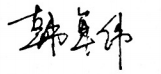
\includegraphics[scale=0.7]{./moderncv/signature.png}\\
\today, Stuttgart

\end{document}
